\section{Estructura Regional y sus Nodos}

\begin{frame}{Estructura Regional: Nodos y Subcentros}
  \begin{columns}[T]
    \begin{column}{0.55\textwidth}
      \begin{itemize}
        \item La región se organiza internamente mediante \termino{nodos urbanos}, 
            puntos que concentran población, servicios y empleo.
        \item \textbf{Nodo Principal:} La CDMX actúa como centro político y 
            administrativo dominante.
        \item \textbf{Subcentros Metropolitanos:} Nodos secundarios como \textit{Santa Fe, Naucalpan o Tlalnepantla} 
            que desconcentran funciones y redistribuyen flujos.
      \end{itemize}
    \end{column}
    \begin{column}{0.40\textwidth}
      \begin{block}{Policentrismo}
        La ciudad contemporánea transita de un modelo centralista a uno de \textbf{núcleos múltiples}, 
        donde subcentros estructuran el territorio de forma independiente.
      \end{block}
    \end{column}
  \end{columns}
\end{frame}

% ── Frame: Tres imágenes con texto explicativo ────────────────────────────────
\begin{frame}{Modelo de Expansión}
  \begin{columns}[T]
    \begin{column}{0.32\textwidth}
      \centering
      \begin{alertblock}{\scriptsize Fase 1: Nodo en expansión}
        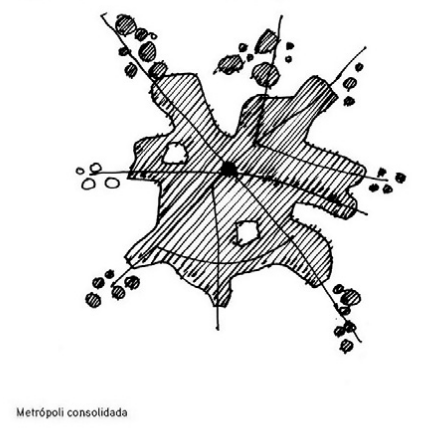
\includegraphics[width=\textwidth, height=3.5cm, keepaspectratio]{img/dispersion_diagrama_3.png}
        \scriptsize\texttt{
            \\
            La ciudad contiene áreas periféricas definidas, pero estos no son nodos, si no 
            extensiones del centro.
        }
      \end{alertblock}
      {\scriptsize
      \fuentefigura{\cite{padilla2022expansion}}            
      .}\\[0.05cm]
    \end{column}

    \begin{column}{0.32\textwidth}
      \centering
      \begin{alertblock}{\scriptsize Fase 2: Nodo en conección}
        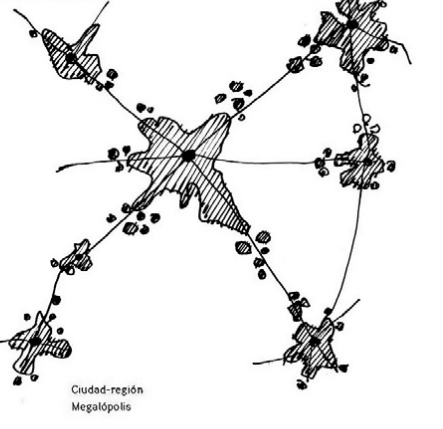
\includegraphics[width=\textwidth, height=3.5cm, keepaspectratio]{img/dispersion_diagrama_4.png}
        \scriptsize\texttt{
            \\
            Los nodos toman fuerza, crean conexiones visibles sus centros hacia sus sus periferias.
        }
      \end{alertblock}
      {\scriptsize
      \fuentefigura{\cite{padilla2022expansion}}
      .}\\[0.05cm]
    \end{column}

    \begin{column}{0.32\textwidth}
      \centering
      \begin{alertblock}{\scriptsize Fase 3: Consolidación }
        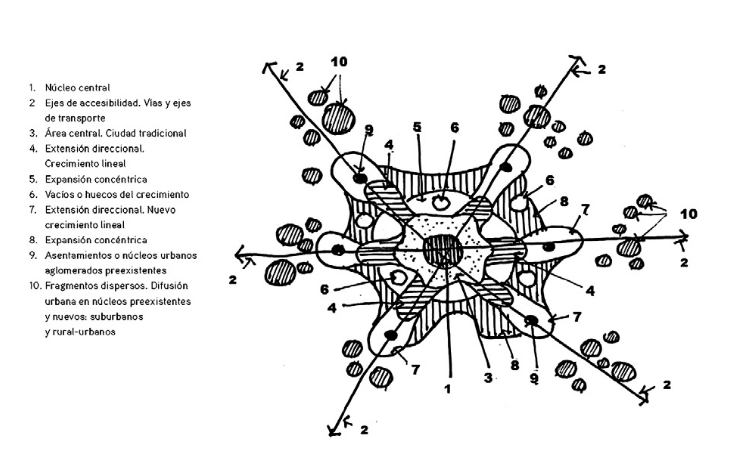
\includegraphics[width=\textwidth, height=3.5cm, keepaspectratio]{img/dispersion_diagrama_1.png}
        \scriptsize\texttt{
            \\
            La región se consolida como una Megalópolis con un nodo central y nodos satelites 
            conectados por diferentes aristas articuladoras. 
        }
      \end{alertblock}
      {\scriptsize
      \fuentefigura{\cite{padilla2022expansion}}
      .}\\[0.05cm]
    \end{column}
  \end{columns}
\end{frame}

\begin{frame}{Estructura Regional: Jerarquías y Subcentros}
  \begin{columns}[T]
    \begin{column}{0.55\textwidth}
      \begin{itemize}
        \item \textbf{Nodo Principal:} La CDMX como centro político, económico y administrativo dominante que concentra 
                servicios especializados.
        \item \textbf{Subcentros Metropolitanos:} Nodos como \textit{Santa Fe, Naucalpan o Tlalnepantla} que desconcentran 
                funciones y redistribuyen flujos.
        \item \textbf{Policentrismo:} Transición hacia un modelo de \termino{núcleos múltiples} donde subcentros estructuran 
                el territorio de forma independiente.
      \end{itemize}
    \end{column}
    \begin{column}{0.35\textwidth}
      \begin{block}{Analogía Sistema Solar}
                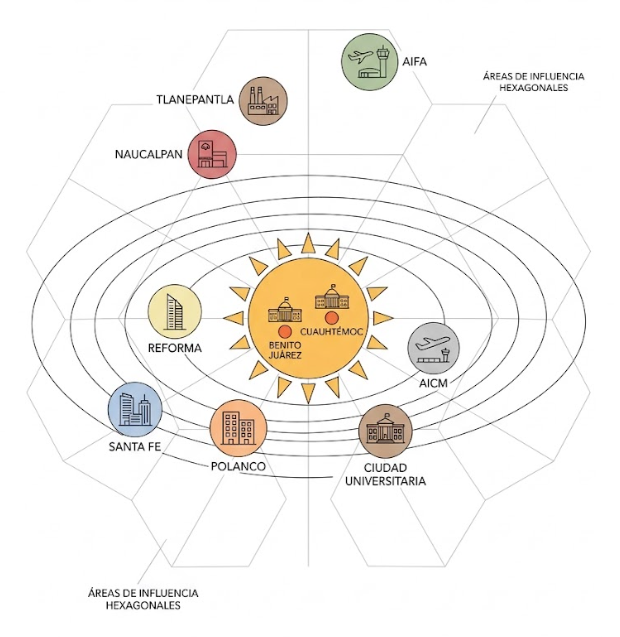
\includegraphics[width=\textwidth, height=5.0 cm]{img/EsquemaCentral.png}
      \end{block}
    \end{column}
  \end{columns}
\end{frame}

\begin{frame}{Corredores Territoriales y el Reto Periférico}
  \begin{itemize}
    \item \textbf{Periferias Dormitorio:} Zonas como \textit{Chimalhuacán o Zumpango} con alta dependencia del nodo central y largos tiempos de traslado 
          \cite{secretaria_economia_datamexico}.
    \item \textbf{Mosaico de Retículas Desfasadas:} La periferia no es una extensión ordenada, sino un "patchwork" de fragmentos geométricamente aislados.
  \end{itemize}
  \begin{alertblock}{Vulnerabilidad Funcional}
    La dependencia de arterias radiales obliga a los usuarios del cuarto contorno a traslados de \textbf{122 minutos}, elevando el \termino{Índice de Ruta Directa (DI)}.
  \end{alertblock}
\end{frame}

\begin{frame}{Reto Periférico Ejemplo}
  \begin{columns}[c] % Alineación vertical al centro
    
    % ========== COLUMNA IZQUIERDA: TABLA ==========
    \begin{column}{0.60\textwidth}
      \begin{table}[htbp]
        \centering
        \caption{\small Caso 7: Santa Catarina en Tláhuac a Ciudad Universitaria}
        \label{tab:conectividad_caso7}
        \smallskip
        % Reducimos el tamaño de la fuente para que quepa verticalmente
        \scriptsize 
        % Ajustamos horizontalmente al ancho de la columna
        \resizebox{\textwidth}{!}{
          \begin{tabular}{ll}
          \toprule
          \textbf{Métrica} & \textbf{Valor} \\
          \midrule
          Punto Abordaje & Eje 10 Sur - Fábrica de Tubos \\
          Punto Descenso & Facultad de Ingeniería \\
          Factor Desviación & 1.82 \\
          Distancia en Red & 42.06 km \\
          Distancia Haversine & 23.10 km \\
          Tiempo en Red & 2.10 h (2 h 6 min) \\
          Tiempo Teórico & 1.15 h (1 h 9 min) \\
          Caminata Total & 0 metros \\
          \bottomrule
          \end{tabular}
        }
      \end{table}
    \end{column}

    % ========== COLUMNA DERECHA: IMAGEN ==========
    \begin{column}{0.38\textwidth}
      \begin{figure}[htbp]
        \centering
        % Reemplaza "esquema_conectividad.png" con el nombre real de tu imagen
        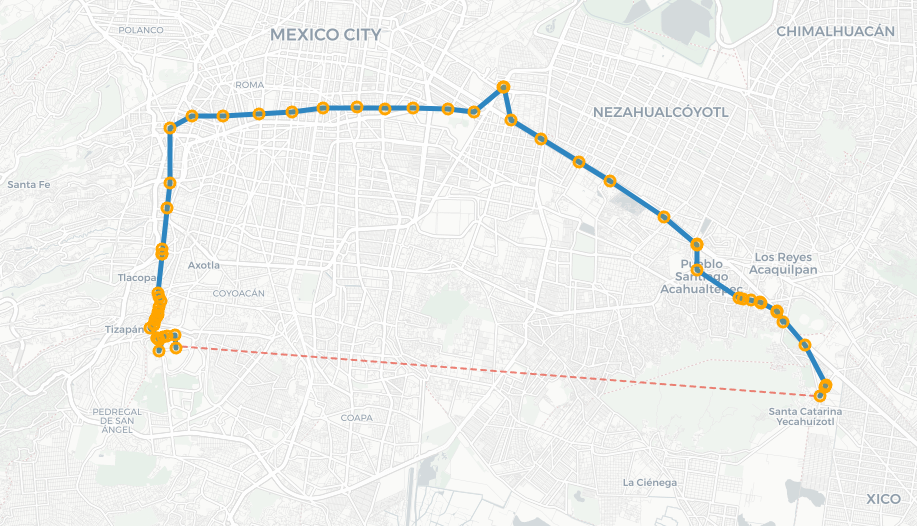
\includegraphics[width=\textwidth, height=0.6\textheight, keepaspectratio]{img/RutaOrienteDF.png}
        \caption{\small Esquema del trayecto. \cite{garibaldi2023vft}}
        \label{fig:esquema_caso7}
      \end{figure}
    \end{column}

  \end{columns}
\end{frame}
